% This text is proprietary.
% It's a part of presentation made by myself.
% It may not used commercial.
% The noncommercial use such as private and study is free
% Sep. 2005 
% Author: Sascha Frank 
% University Freiburg 
% www.informatik.uni-freiburg.de/~frank/


\documentclass{beamer}
\usetheme{Copenhagen}

\usecolortheme{beaver}
\begin{document}

%\logo{
\includegraphics[height=0.5cm]{cet.jpg}} 

\title{{\bf A}sterisk {\bf R}ad{\bf I}o {\bf A}rchetecture}
\subtitle{\it VoIP Based Campus Announcment System}  
\author{Dhananjay M Balan} 
\institute[College Of Engineering] % (optional)
{
  College Of Engineering, Trivandrum\\
  University Of Kerala.
}
\date{\today} 

\frame{\titlepage
\centerline{
\includegraphics[height=2cm]{cet.jpg}}} 

\frame{\frametitle{Table of contents}\tableofcontents} 

\section{Introduction}
\subsection{Problem}

\frame{
\frametitle{Problem}
\bf{ \large A geographically large campus with many groups of students have to implement an announcment system.}

}

\frame{
\frametitle{Conventional System}
\begin{enumerate}
 \item No {\bf Flexibility} in selection of audiance. \pause
 \item Requires {\bf heavy cableing} around the campus. \pause
 \item Limted {\bf scalability and extentability}. \pause
\end{enumerate}
}

\subsection{Solution}

\frame{
  \frametitle{VoIP}
  {\it{\bf VoIP} is a family of technologies, methodologies, communication protocols, and transmission techniques for the delivery of voice communications and multimedia sessions over Internet Protocol (IP) networks, such as the Internet.}\\
  
  \hfill{\bf - Wikipedia.org, Accesed \today}
  }
  
\frame{
  \frametitle{Advantages}
    \begin{enumerate}
     \item Each client can be addressed individually. \pause
     \item Can utilize the existing IP network in campus. \pause
     \item Scalable - Adding a new client is simple as long as there is network connectivity - No load problems. \pause
     \item Have an option to build interactive systems. \pause
     \item Provision for remote access. \pause
     \item Easy modification of plans - No hard circutes. \pause
    \end{enumerate}
    }

\frame{   
  \frametitle{Products Currently Available}
  \begin{enumerate}
   \item xyz 
  \end{enumerate}
{\bf No Free Software} products exist, Though almost all core components are available in a compatible licence.   
}

%\section{ARIA System.}

\frame{
  \frametitle{Block Diagram}
  \centerline{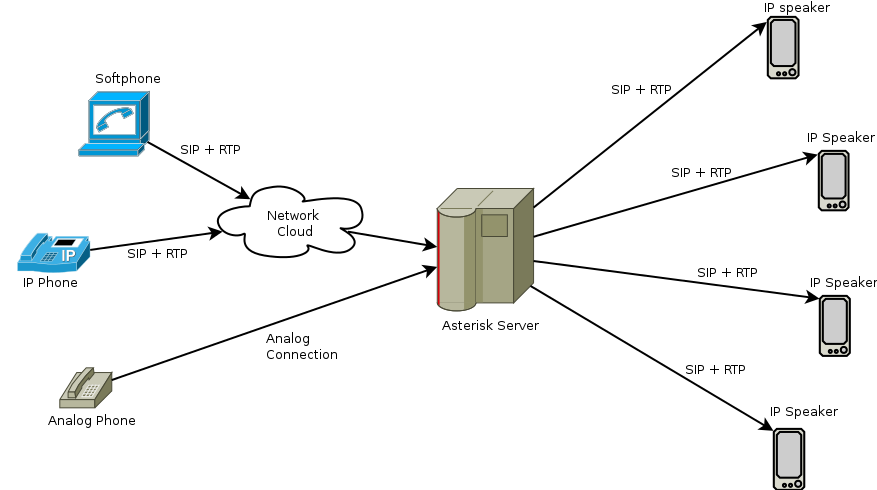
\includegraphics[width=\textwidth]{functional_diagram.png}}
  }
  \subsection{Tools}

  
  \frame{
    \frametitle{Protocols}
    \begin{enumerate}
     \item The {\bf Session Initiation Protocol (SIP)} is an IETF-defined signaling protocol widely used for controlling communication sessions such as voice and video calls over Internet Protocol (IP). The protocol can be used for creating, modifying and terminating two-party (unicast) or multiparty (multicast) sessions. \pause
    
    \item {\bf RTP} provides end-to-end network transport functions suitable for applications transmitting real-time data, such as audio, video or simulation data, over multicast or unicast network services. {\it (RFC 3550)}
    \end{enumerate}
    }

\frame{
  \frametitle{Asterisk}
  \hfill{
\includegraphics[scale=0.5]{Asterisk_logo.png}}\\
  {\it {\bf Asterisk} is a software implementation of a telephone private branch exchange (PBX); it was created in 1999 by Mark Spencer of Digium. Like any PBX, it allows attached telephones to make calls to one another, and to connect to other telephone services including the public switched telephone network (PSTN) and Voice over Internet Protocol (VoIP) services. Its name comes from the asterisk symbol, “*”.}\\
  \hfill{{\bf - Wikipedia.org. accessed \today}} \pause
  
  {\bf Asterisk} thus essentialy can act as a SIP proxy for routing the IP multicast trasport we needed to implement.
  
  }
  
\frame{
  \frametitle{Working}
  \centerline{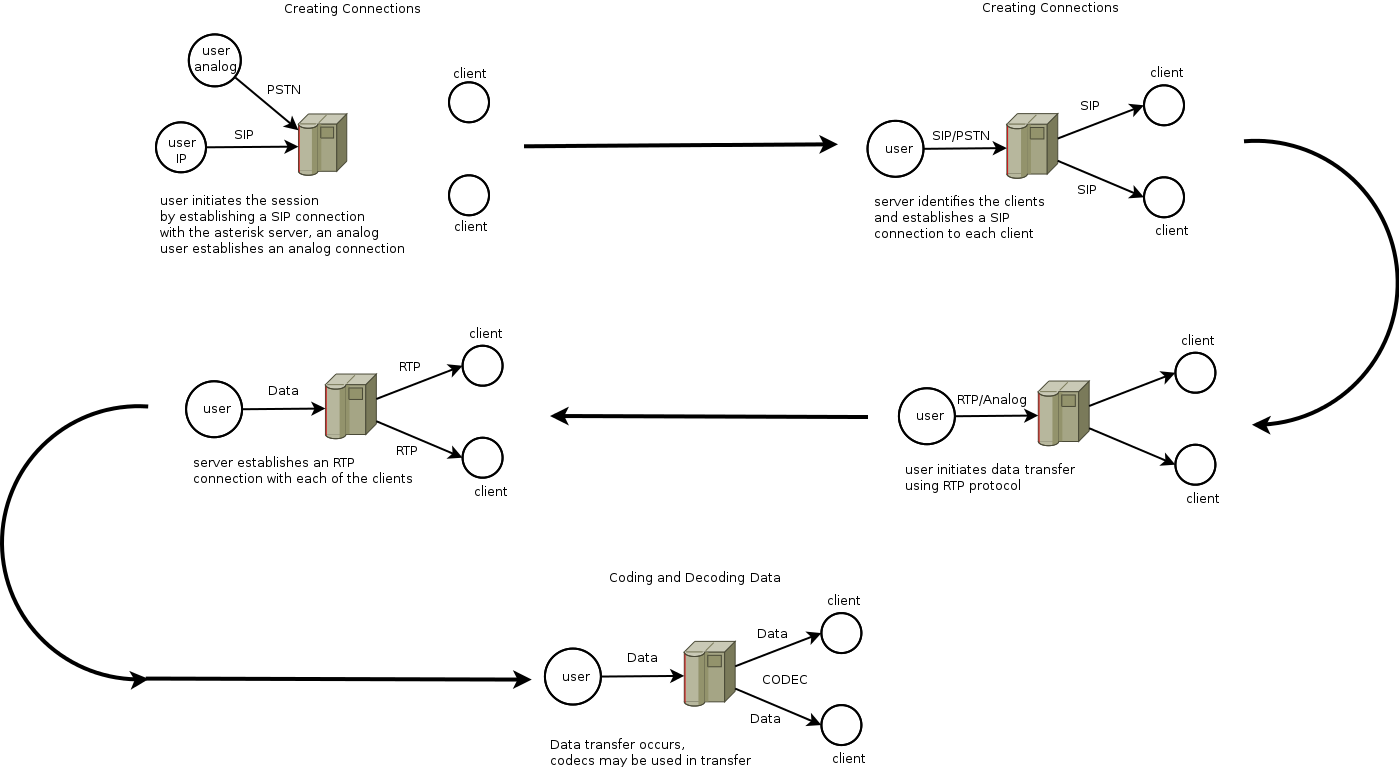
\includegraphics[width=\textwidth]{working.png}}
  }
 \frame{
  \frametitle{Challenges}
  \begin{enumerate}
   \item Development of software for transmission and reciever.
   \item Development of a streamlined aproach for configuring Astrisk PA System.
   \item Implementation and Testing.
  \end{enumerate}
  }
  \frame{
  \frametitle{Expenditure}
  \begin{itemize}
   \item Consumables
   \begin{itemize}
    \item Network equipments Rs. 1500
    \item Import charges on equipment Rs. 7000
    \item Misc Charges: Rs. 1000

   \end{itemize}

   \item Equipments
   \begin{itemize}
      \item IP Phone  Rs. 5000
      \item IP speakers x2 Rs. 10000
      \item Digium FXO cards - 1TDM410PLF Rs. 10000
   \end{itemize}
   
   \item Research Literature - Rs. 3000
   \item Others
   \begin{itemize}
    \item Uplink to telephony provider to test remote link. (college PBX)

   \end{itemize}

   \item Contingencies Rs. 1000.
   \begin{itemize}
    \item Rs. 4000 in case IP speakers are not available.

   \end{itemize}


  \end{itemize}

}  

\end{document}

